\documentclass[border=1pt]{standalone}
% packages
\usepackage{tikz}
\usepackage{tikz-qtree}
\usetikzlibrary{positioning,quotes,calc,arrows.meta,shapes}
% tikz setup
\tikzset{%
  arrow/.style = {
    ->,
    > = latex,
    very thick,
    rounded corners,
    fill = #1,
    draw = #1,
  },
  wide/.style = {
    line width = #1,
  },
  tbox/.style = {
    thick,
    rounded corners,
    fill = #1!20!white,
    draw = #1!80!white,
    align = center,
    minimum width = 0.8cm,
    minimum height = 0.6cm,
    node distance = 1.5cm,
  },
  branch/.style = {
    grow = down,
    thick,
    rounded corners = 0.1cm,
    fill = #1!20!white,
    draw = #1!80!white,
    align = center,
    minimum width = 3cm,
    minimum height = 1cm,
    node distance = 1cm,
  },
  branch/.default = {gray},
  leaf/.style = {
    grow = down,
    thick,
    rounded corners = 0.35cm,
    fill = #1!20!white,
    draw = #1!80!white,
    align = center,
    minimum width = 0.7cm,
    minimum height = 0.7cm,
    font = \normalfont,
  },
  leaf/.default = {blue},
}
% selectors
\definecolor{all}     {RGB}{  0,  0,  0}
\definecolor{S}       {RGB}{  0,153,255}
\definecolor{I}       {RGB}{204, 51,  0}
\definecolor{T}       {RGB}{204, 51,153}
\definecolor{infected}{RGB}{204,  0, 51}
\definecolor{High}    {RGB}{ 34, 34, 34}
\definecolor{Med}     {RGB}{ 85, 85, 85}
\definecolor{Low}     {RGB}{187,187,187}
% from beamer
\definecolor{C1}{HTML}{224466}
\definecolor{C2}{HTML}{CC3300}
\definecolor{C3}{HTML}{666666}

\begin{document}
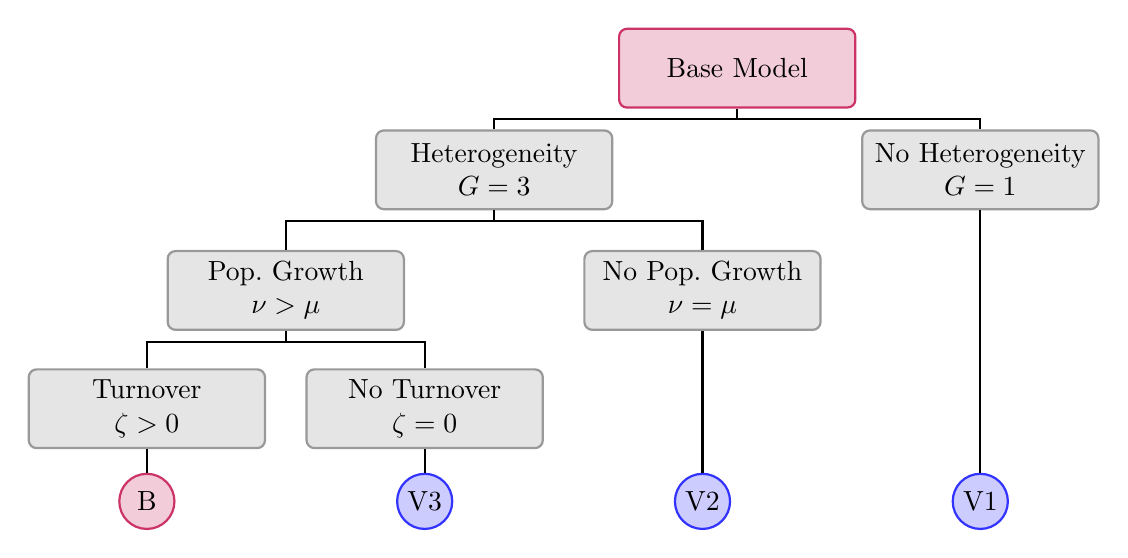
\begin{tikzpicture}[
    level distance = 1.5cm,
    sibling distance = 0.5cm,
    every path/.append style = { thick },
    edge from parent path = {
      (\tikzparentnode) -- +(0.0,-0.65cm) -| (\tikzchildnode)
    },
    frontier/.style = { distance from root = 5.5cm }
  ]
  \Tree
    [.\node[branch=purple]{Base Model};
      [.\node[branch]{Heterogeneity \\ $G=3$};
        [.\node[branch]{Pop.\ Growth \\ $\nu>\mu$};
          [.\node[branch]{Turnover \\ $\zeta > 0$}; \node[leaf=purple]{B}; ]
          [.\node[branch]{No Turnover \\ $\zeta = 0$}; \node[leaf]{V3}; ]
        ]
        [.\node[branch]{No Pop.\ Growth \\ $\nu=\mu$}; \node[leaf]{V2}; ]
      ]
      [.\node[branch]{No Heterogeneity \\ $G=1$}; \node[leaf]{V1}; ]
    ]
\end{tikzpicture}
\end{document}